\begin{activite}[Un p'tit tour dans l'Espace !]

\begin{partie}[Quelques représentations]
\begin{minipage}[c]{0.19\linewidth}
 \begin{center}  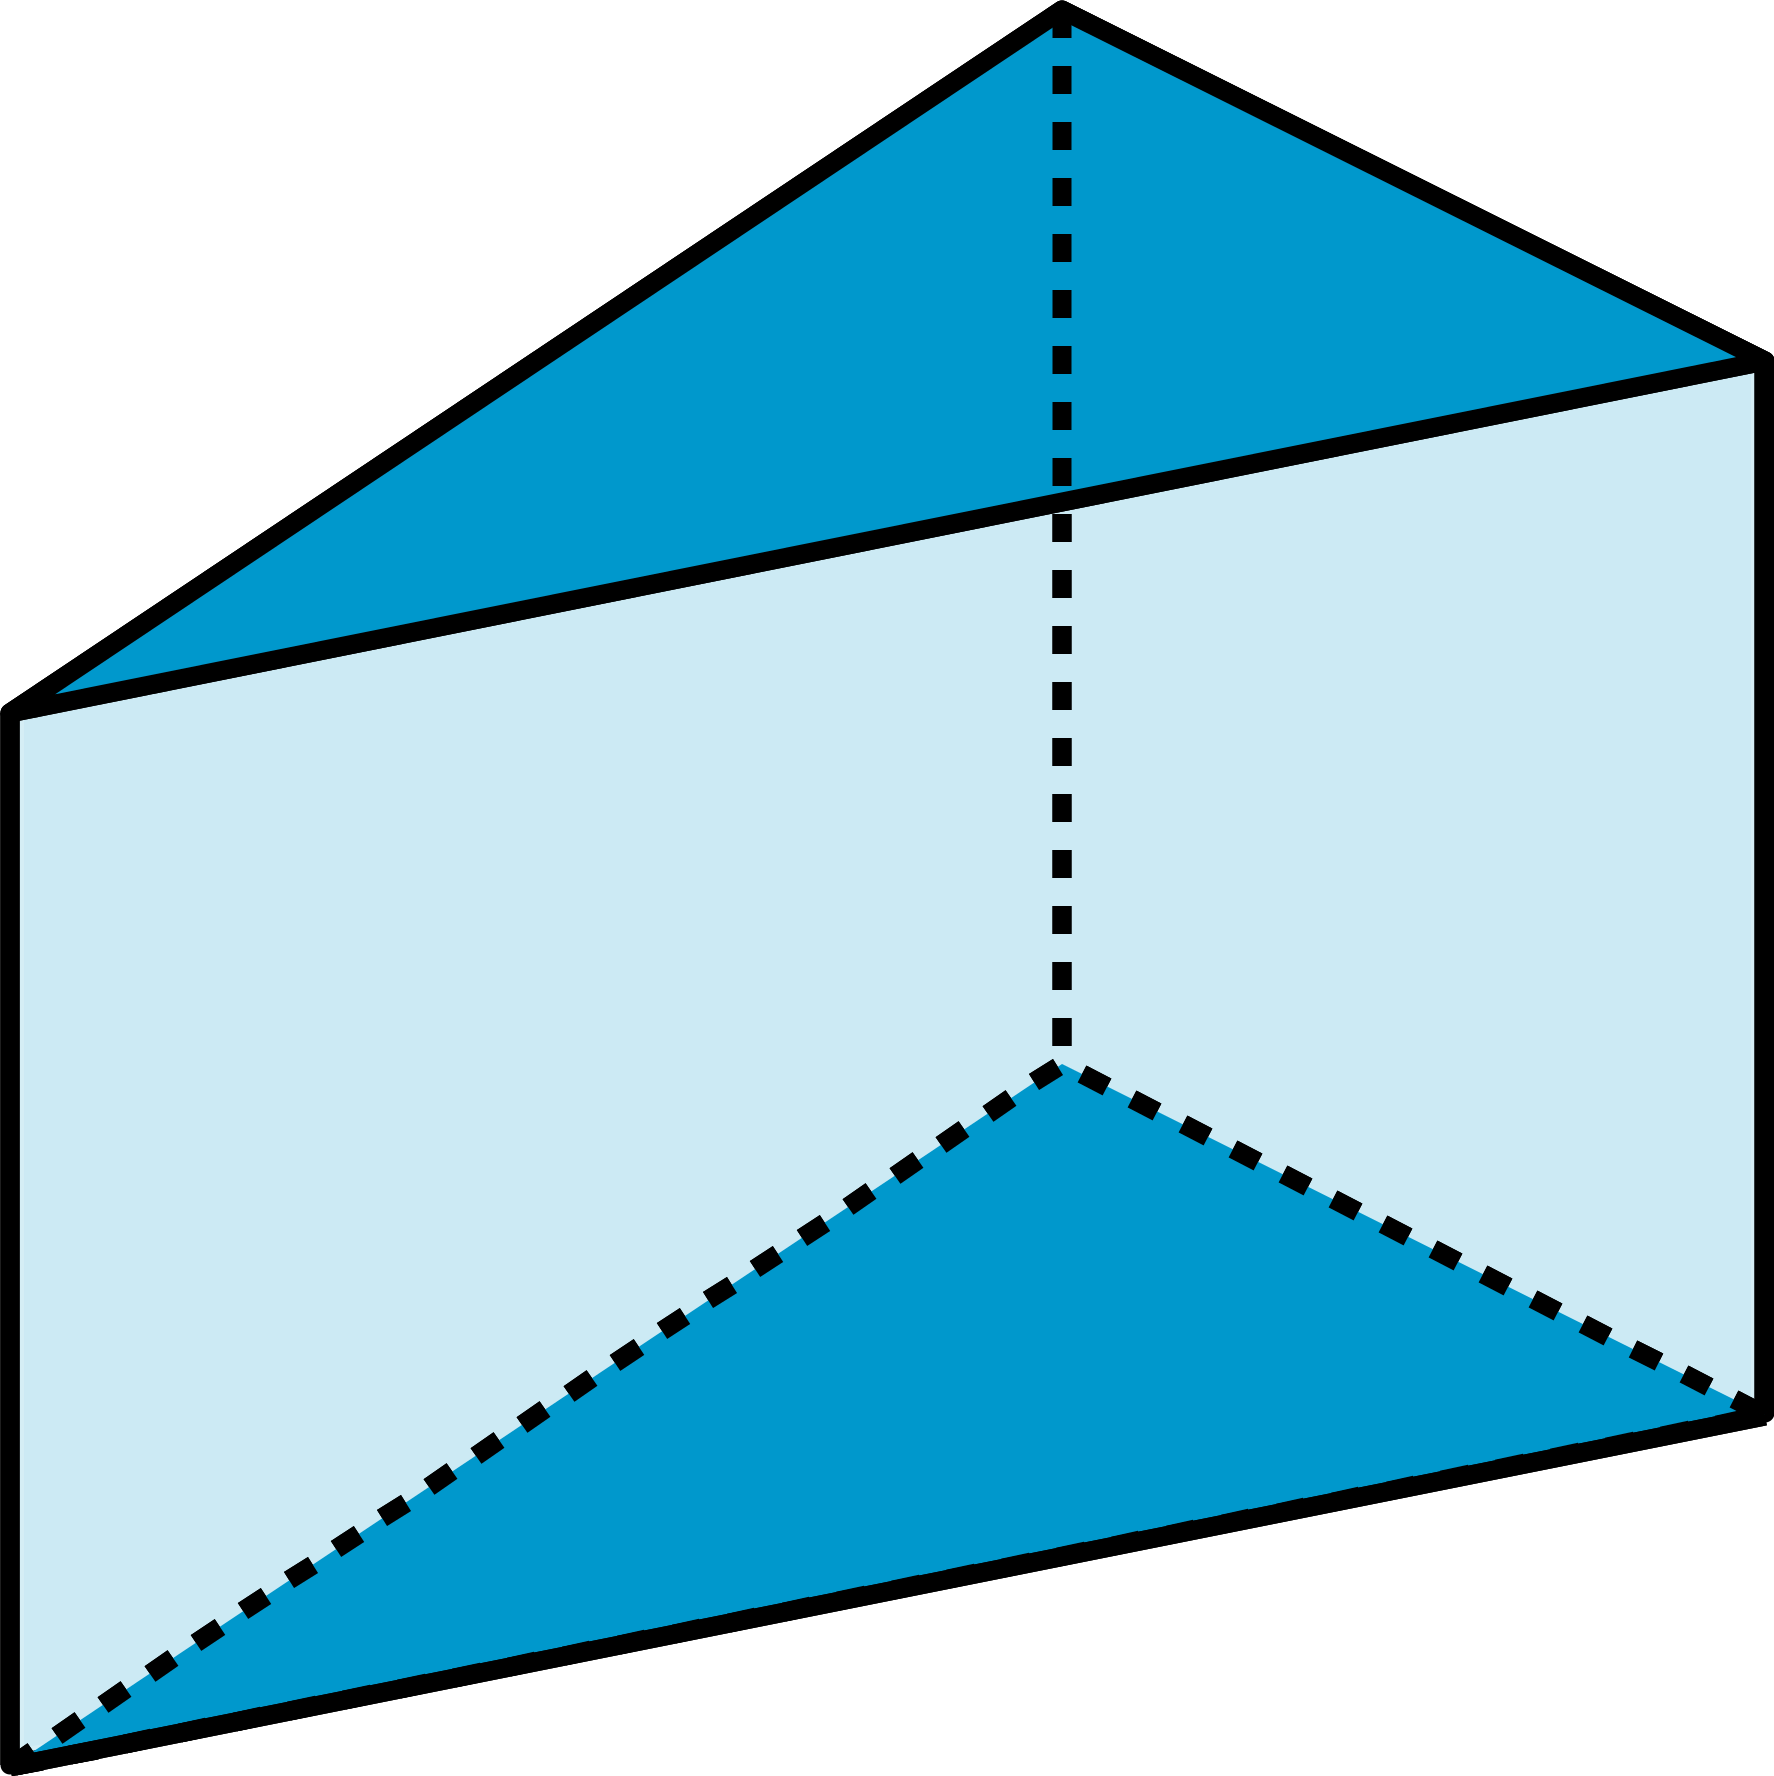
\includegraphics[width=1.9cm]{espace_obj1} \end{center}
 \end{minipage} \hfill%
\begin{minipage}[c]{0.19\linewidth}
 \begin{center}  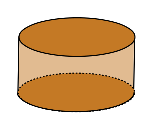
\includegraphics[width=2.1cm]{espace_obj2} \end{center}
 \end{minipage} \hfill%
\begin{minipage}[c]{0.19\linewidth}
 \begin{center}  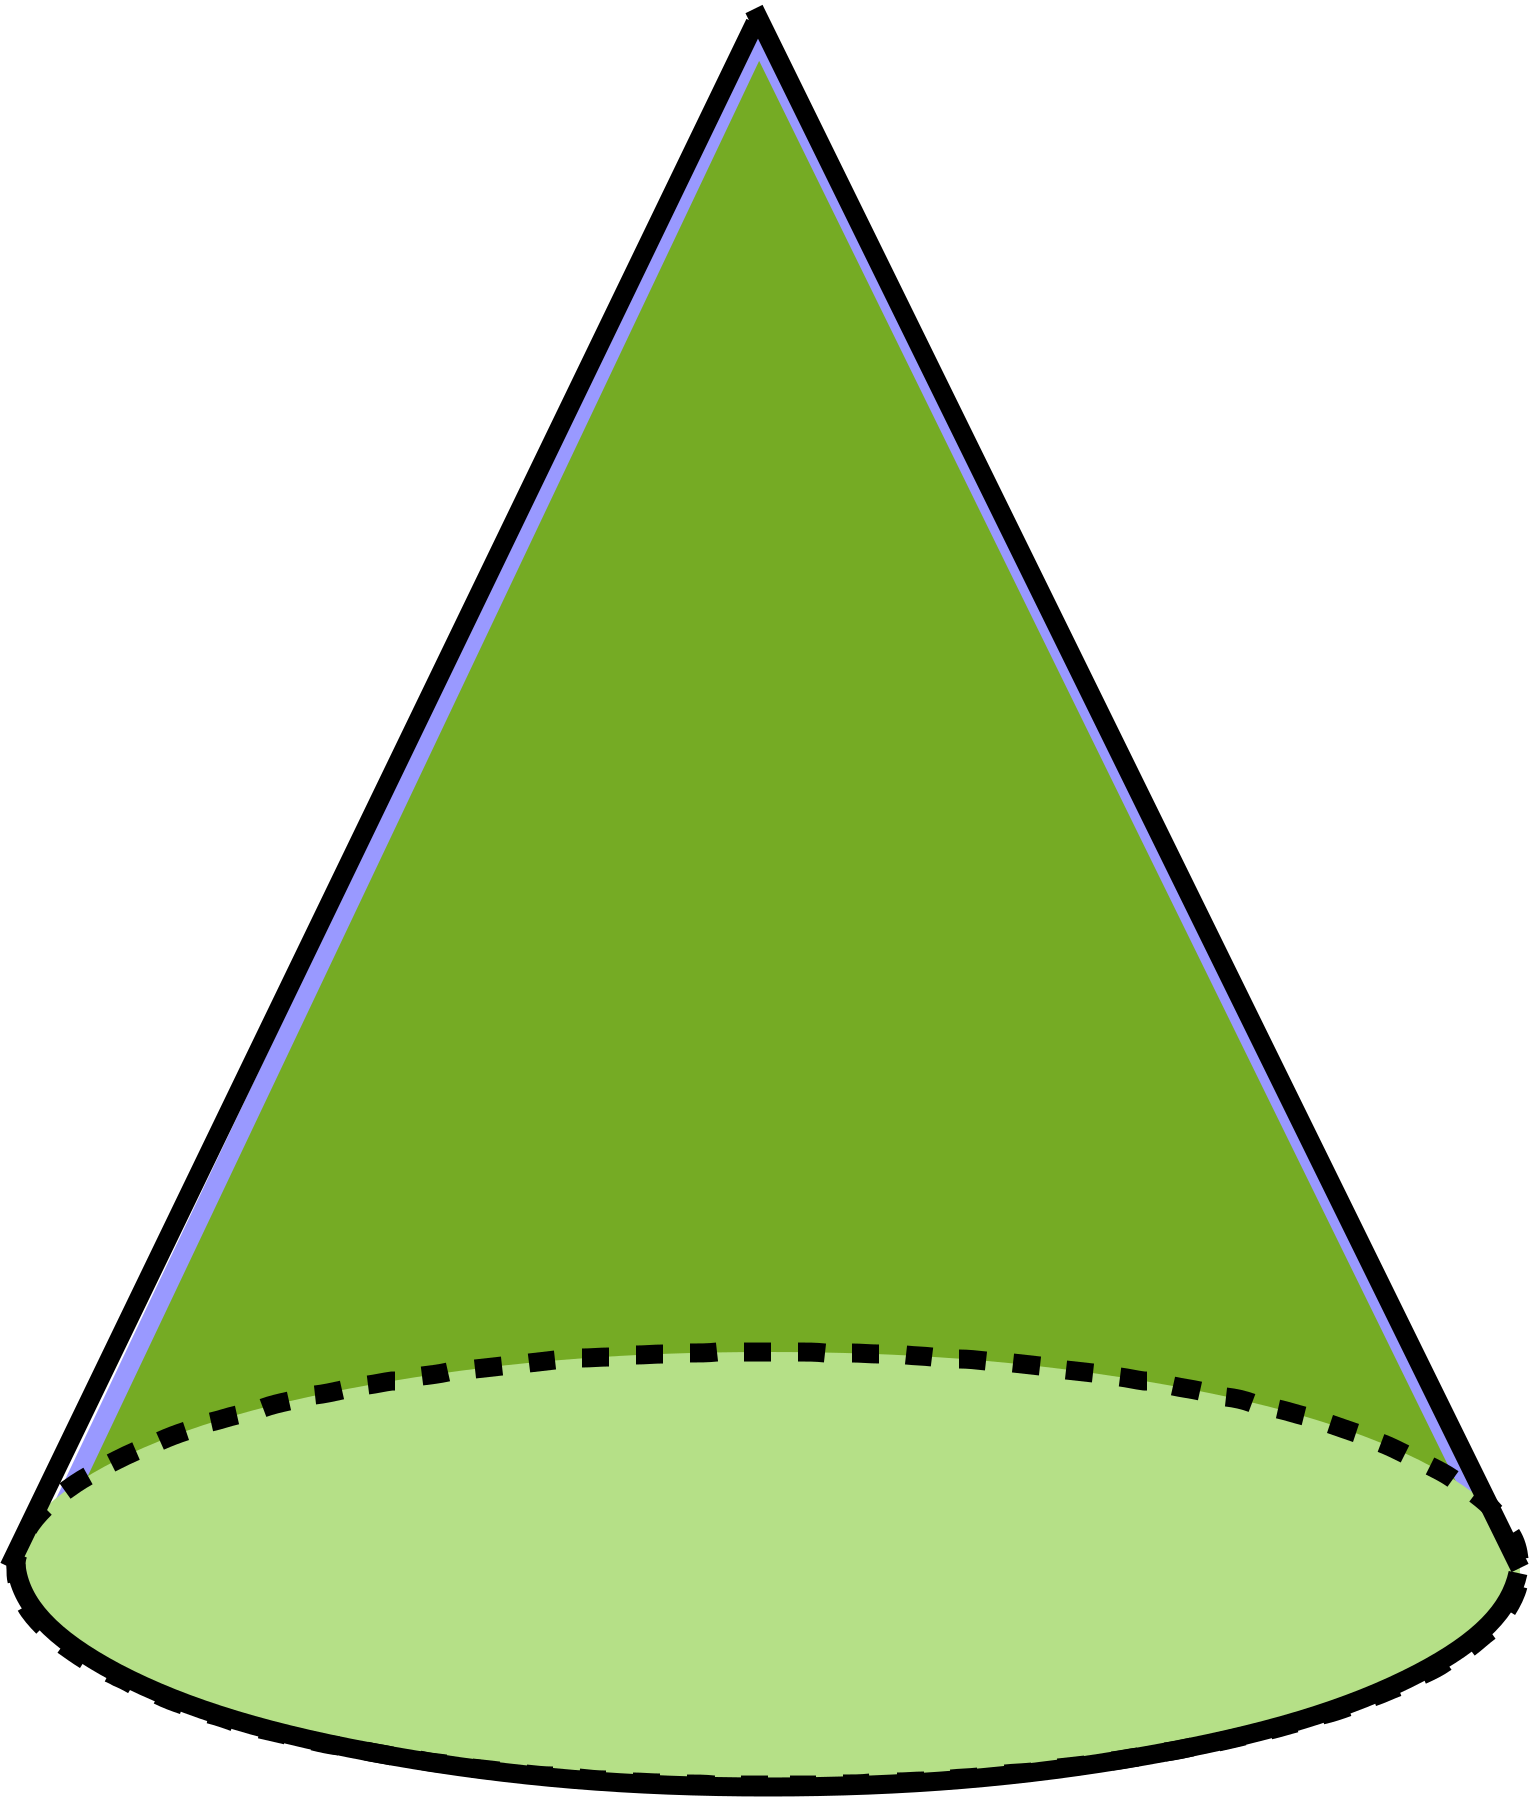
\includegraphics[width=1.6cm]{espace_obj3} \end{center}
 \end{minipage} \hfill%
\begin{minipage}[c]{0.19\linewidth}
 \begin{center}  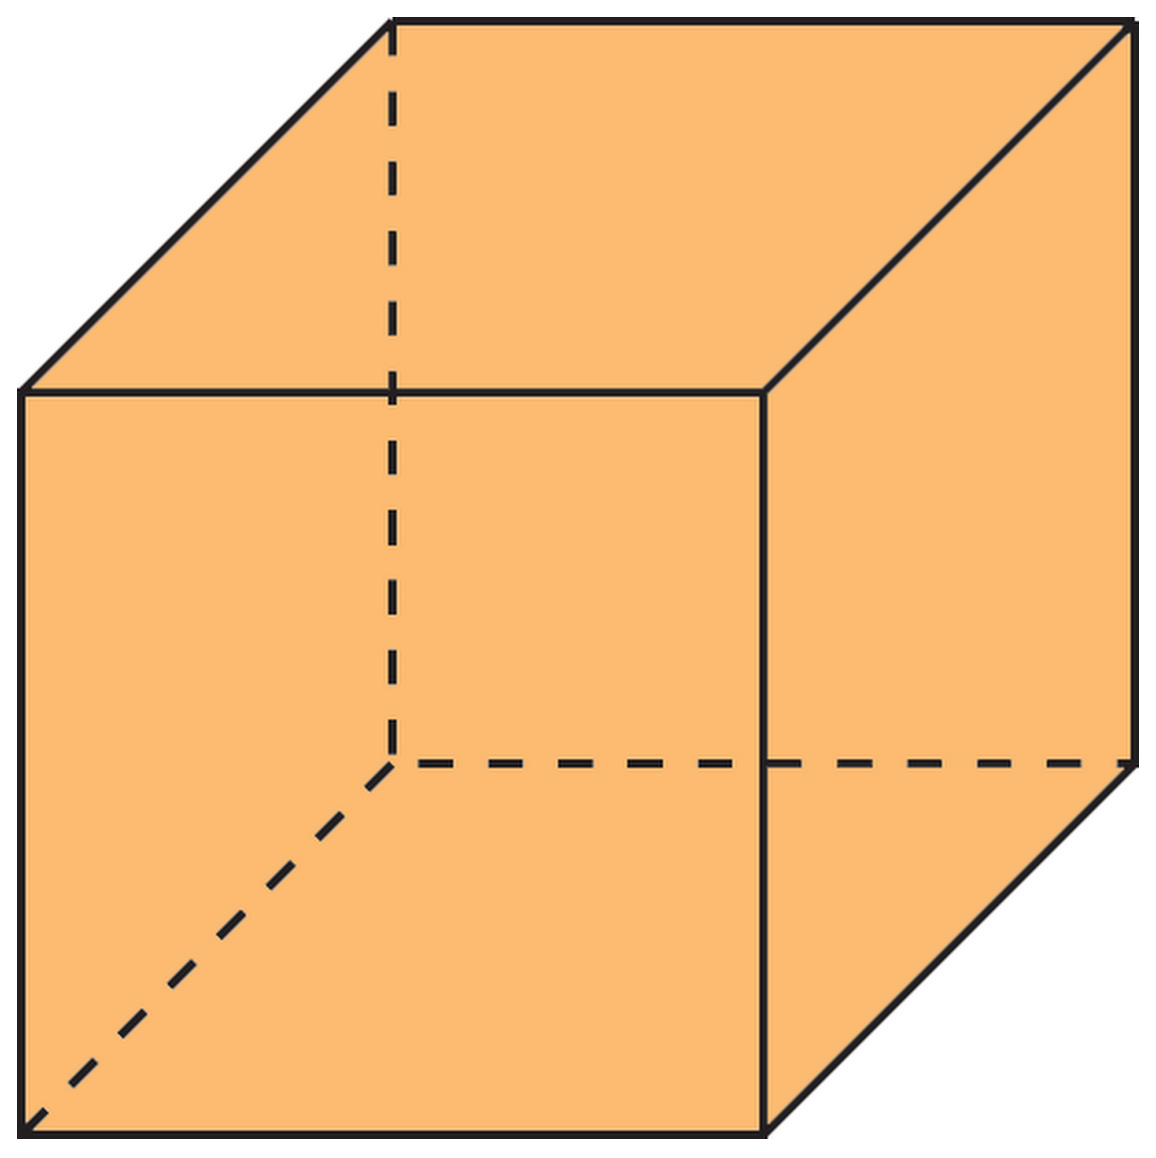
\includegraphics[width=2.1cm]{espace_obj4} \end{center}
 \end{minipage} \hfill%
\begin{minipage}[c]{0.19\linewidth}
 \begin{center}  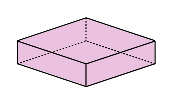
\includegraphics[width=2.5cm]{espace_obj5} \end{center}
 \end{minipage} \\
 
\begin{minipage}[c]{0.19\linewidth}
\begin{center} objet 1 \end{center}
 \end{minipage} \hfill%
\begin{minipage}[c]{0.19\linewidth}
 \begin{center} objet 2 \end{center}
 \end{minipage} \hfill%
\begin{minipage}[c]{0.19\linewidth}
\begin{center} objet 3 \end{center}
 \end{minipage} \hfill%
\begin{minipage}[c]{0.19\linewidth}
\begin{center} objet 4 \end{center}
 \end{minipage} \hfill%
\begin{minipage}[c]{0.19\linewidth}
\begin{center} objet 5 \end{center}
 \end{minipage} \\
\begin{enumerate}
 \item À quels objets de la vie courante te font penser les objets ci‑dessus ?
 \item Pourquoi y a‑t‑il des traits en pointillés ?
 \item Pour les \emph{objets 1}, \emph{4} et \emph{5}, indique le nombre de \textbf{faces}, d'\textbf{arêtes} et de \textbf{sommets}.
 \item Pour chaque objet, dessine à main levée une représentation possible de la vue de dessus.
 \item Dans la réalité, les faces de l'\emph{objet 5} sont des rectangles. Qu'en est‑il dans sa représentation ci‑dessus ?
 \end{enumerate}
\end{partie}

\begin{partie}[Perspective cavalière]
\begin{minipage}[c]{0.58\linewidth}
\begin{enumerate}
 \item Plusieurs perspectives existent. Celle de l'objet 5 est appelée perspective dimétrique. On veut le représenter en \textbf{perspective cavalière} dont une particularité est d'avoir une face en vraie grandeur. On a commencé son tracé. Reproduis‑le et complète‑le en utilisant le quadrillage.
 \item Représente maintenant un cube en perspective cavalière en prenant cinq carreaux pour côté du carré en vraie grandeur. 
 \end{enumerate}
 \end{minipage} \hfill%
 \begin{minipage}[t]{0.38\linewidth}
  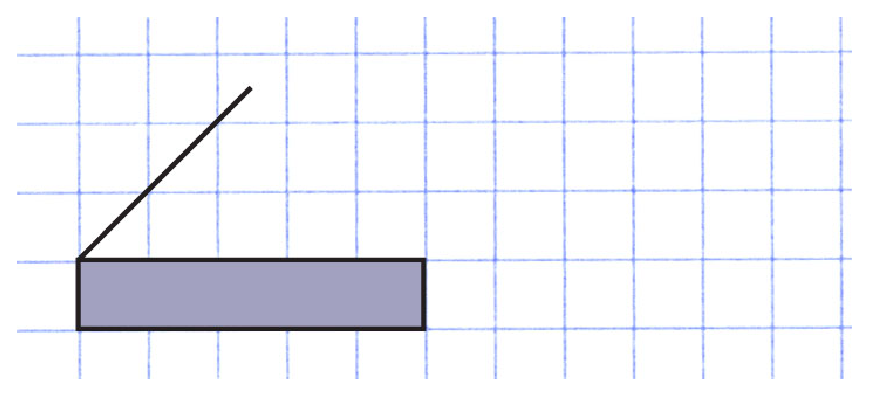
\includegraphics[width=5.5cm]{cavaliere}
  \end{minipage} \\
\end{partie}

\end{activite}

%%%%%%%%%%%%%%%%%%%%%%%%%%%%%%%%%%%%%%%%%%%%%%%%%%%%%%%%%%%%%%%%%%%%%%%%%%

\begin{activite}[De l'enveloppe au cube]

\begin{partie}[Préparation de l'enveloppe]
\begin{enumerate}
 \item Achète une enveloppe standard de format 11 cm × 22 cm et plie‑la en deux de façon à obtenir un carré (figure 1).
 \item Repère le centre d'un carré au crayon (figure 2). 
 \item Ramène les sommets du carré vers le centre en marquant bien les plis des deux côtés (figures 3 et 4). Déplie, tu dois obtenir la figure 5.
 \end{enumerate}
\begin{minipage}[c]{0.21\linewidth}
 \begin{center}  
\includegraphics[width=2.4cm]{enveloppe_c1} \end{center}
 \end{minipage} \hfill%
\begin{minipage}[c]{0.21\linewidth}
 \begin{center}  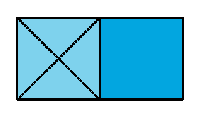
\includegraphics[width=2.4cm]{enveloppe_c2} \end{center}
 \end{minipage} \hfill%
\begin{minipage}[c]{0.16\linewidth}
 \begin{center}  
\includegraphics[width=1.2cm]{enveloppe_c3} \end{center}
 \end{minipage} \hfill%
\begin{minipage}[c]{0.16\linewidth}
 \begin{center}  
\includegraphics[width=1.5cm]{enveloppe_c4} \end{center}
 \end{minipage} \hfill%
\begin{minipage}[c]{0.21\linewidth}
 \begin{center}  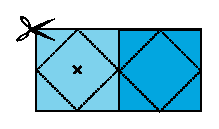
\includegraphics[width=2.6cm]{enveloppe_c5} \end{center}
 \end{minipage} \\
 
\begin{minipage}[c]{0.19\linewidth}
\begin{center} figure 1 \end{center}
 \end{minipage} \hfill%
\begin{minipage}[c]{0.19\linewidth}
 \begin{center} \qquad figure 2 \end{center}
 \end{minipage} \hfill%
\begin{minipage}[c]{0.19\linewidth}
\begin{center} \qquad figure 3 \end{center}
 \end{minipage} \hfill%
\begin{minipage}[c]{0.19\linewidth}
\begin{center} figure 4 \end{center}
 \end{minipage} \hfill%
\begin{minipage}[c]{0.19\linewidth}
\begin{center} figure 5 \end{center}
 \end{minipage} \\
\end{partie}

\begin{partie}[Abracadabra !]
Découpe le haut de l'enveloppe pour l'ouvrir (figure 5). En ouvrant l'enveloppe, tu dois voir apparaître un cube !  \\[0.5em]
Colle cette enveloppe dans une double page de ton cahier de façon à ce que le cube se reforme quand tu ouvres ton cahier au niveau de cette double page.
\end{partie}

\end{activite}

%%%%%%%%%%%%%%%%%%%%%%%%%%%%%%%%%%%%%%%%%%%%%%%%%%%%%%%%%%%%%%%%%%%%%%%%%%

\begin{activite}[La chasse aux cubes]

\begin{partie}[Pour commencer \ldots]
\begin{minipage}[c]{0.58\linewidth}
Julien dispose d'un jeu de cubes tels que celui‑ci : 
 \end{minipage} \hfill%
\begin{minipage}[c]{0.38\linewidth}
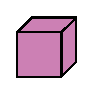
\includegraphics[width=1.2cm]{chasse_c1}
 \end{minipage} \\
\begin{minipage}[c]{0.7\linewidth}
En assemblant six de ces cubes, il obtient un nouveau solide : 
 \end{minipage} \hfill%
\begin{minipage}[c]{0.26\linewidth}
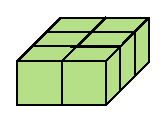
\includegraphics[width=2.2cm]{chasse_c2}
 \end{minipage} \\
\begin{enumerate}
 \item Comment s'appelle ce solide ?
 \item Combien a‑t‑il de faces ? Donne la nature de chaque face. Combien y en a‑t‑il de différentes tailles ? Dessine chacune d'elles en vraie grandeur sachant que l'arête du petit cube est 1 cm.
 \item Dessine ce solide en perspective cavalière et colorie deux de ses faces parallèles. Au total, combien y a‑t‑il de paires de faces parallèles ?
 \end{enumerate}
\end{partie}

\begin{partie}[Un peu plus dur \ldots]
\begin{enumerate}
 \item Avec huit cubes, combien peut‑on construire de \textbf{pavés droits} différents ?
 \item Dessine en perspective cavalière et à main levée tous les solides obtenus. (Tu pourras t'aider de papier pointé.) Est‑ce que certains sont « plus particuliers » que d'autres ?
 \item Quel(s) est (sont) celui (ceux) qui a (ont) la plus grande arête ? La plus petite arête ?
 \item Quel(s) est (sont) celui (ceux) qui a (ont) la plus grande face ? La plus petite face ?
 \item Ont‑ils tous le même nombre de sommets ?
 \end{enumerate}
\end{partie}

\end{activite}

%%%%%%%%%%%%%%%%%%%%%%%%%%%%%%%%%%%%%%%%%%%%%%%%%%%%%%%%%%%%%%%%%%%%%%%%%%

\begin{activite}[Patron du pavé droit]

\begin{partie}[Dimensions de la boîte]
Gilles a sous les yeux une boîte qu'il voudrait reconstruire à l'identique, en papier. Cette boîte a la forme d'un pavé droit. 
\begin{enumerate}
 \item Il mesure les côtés d'une face et trouve 2,5 cm et 3,5 cm. Reproduis cette face en grandeur réelle sur ton cahier.
 \item Il mesure une autre face et constate qu'elle a la même largeur que la première et qu'elle est deux fois plus longue. Reproduis cette seconde face.
 \item Malheureusement, il n'a pas le temps de prendre d'autres mesures et doit rentrer chez lui. Avec ce qu'il a pu mesurer, a‑t‑il toutes les informations pour reconstruire la boîte ? Si oui, donne les dimensions de la troisième face et reproduis-la.
 \end{enumerate}
\end{partie}

\begin{partie}[Vers le patron]
\begin{enumerate}
 \item Construis un \textbf{patron} possible de ce pavé droit. Y a‑t‑il plusieurs possibilités ?
 \item Découpe et assemble le patron.
 \end{enumerate}
\end{partie}

\begin{partie}[Emballer c'est peser]
\begin{minipage}[c]{0.78\linewidth}
 \begin{enumerate}
  \item On utilise du ruban pour ficeler cette boîte. Sachant qu'il en faut 9 cm pour le nœud, quelle est la longueur de ruban nécessaire ?
  \item Il y a deux autres façons de la ficeler. Pour chacune, fais un schéma et calcule la longueur de ruban nécessaire.
  \item Quelle est la méthode qui nécessite le moins de ruban ?
 \end{enumerate}
\end{minipage} \hfill%
\begin{minipage}[c]{0.18\linewidth}
 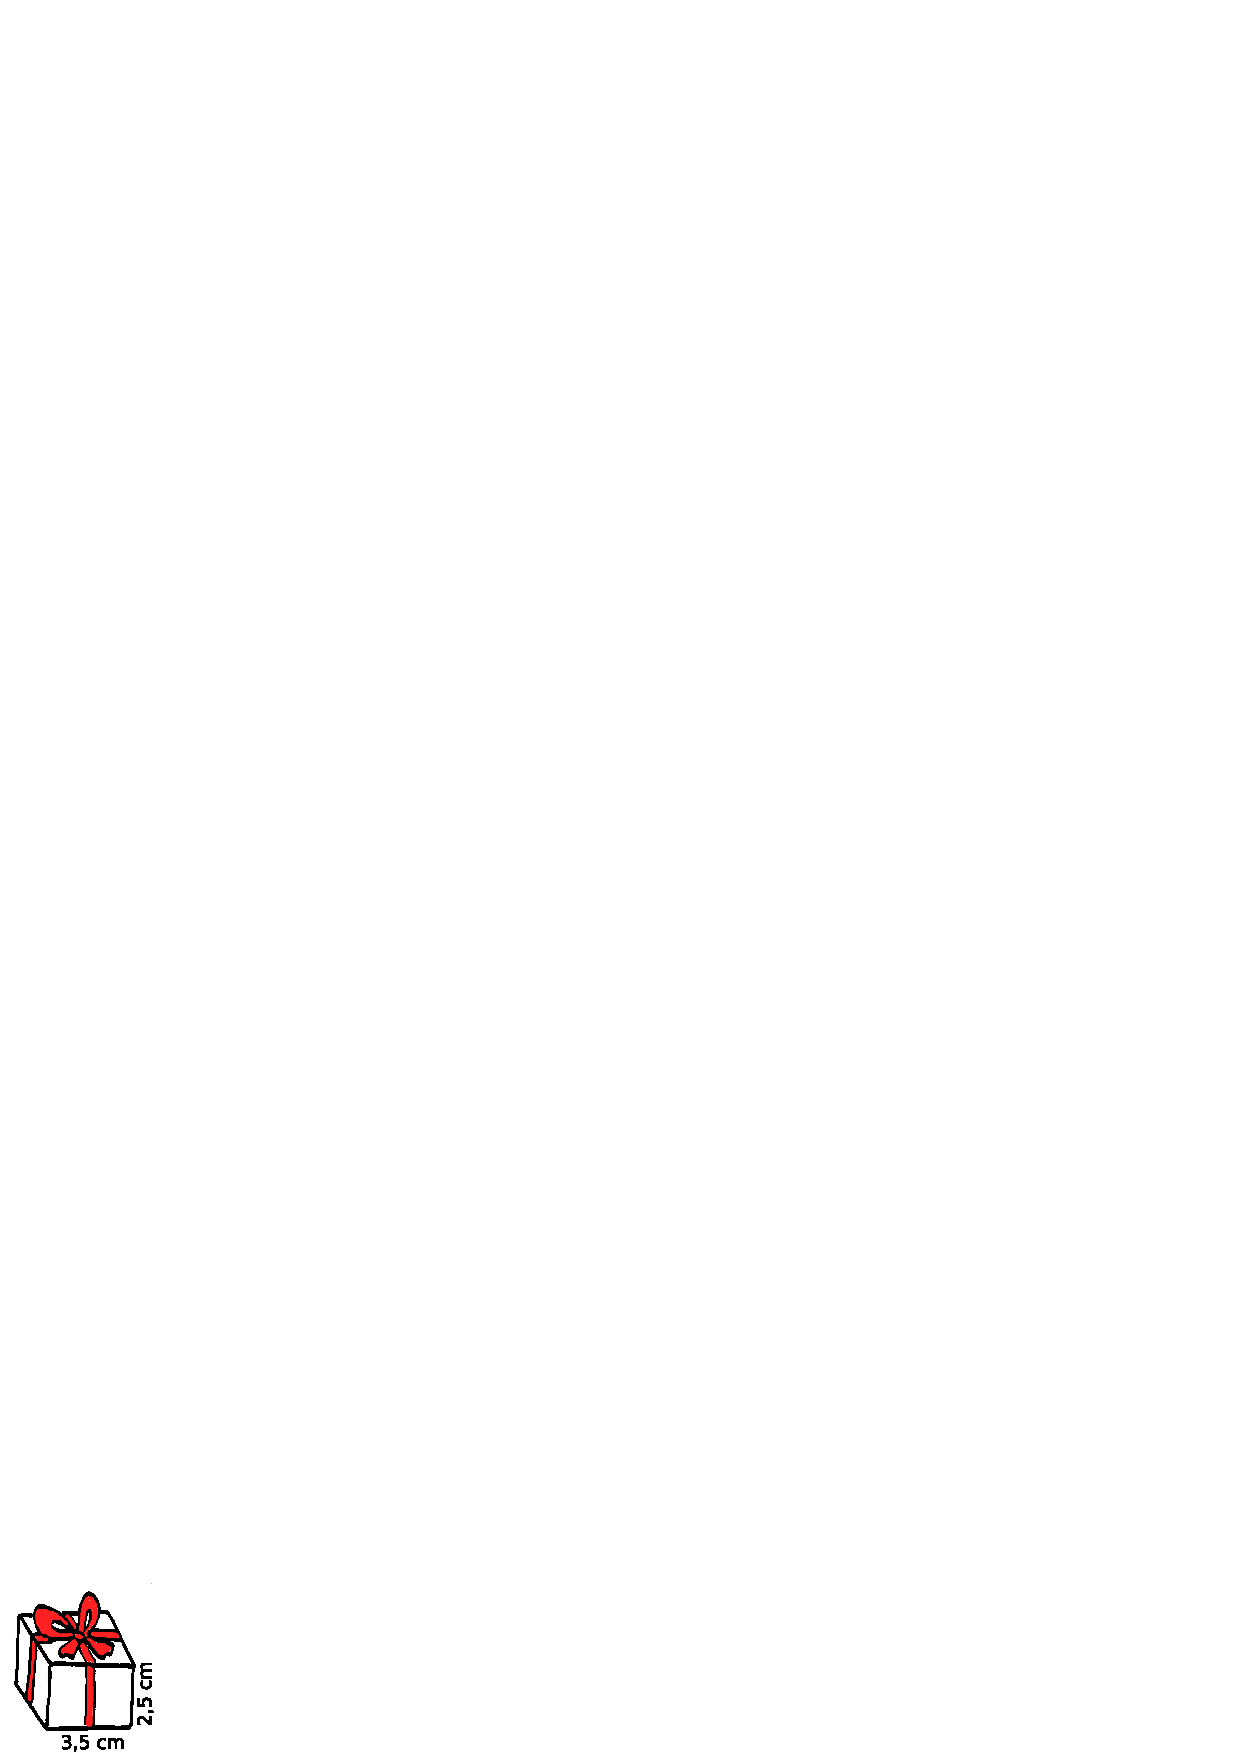
\includegraphics[width=2.5cm]{cadeau_emballage}
\end{minipage} \\
\end{partie}

\end{activite}

%%%%%%%%%%%%%%%%%%%%%%%%%%%%%%%%%%%%%%%%%%%%%%%%%%%%%%%%%%%%%%%%%%%%%%%%%%

\begin{activite}[Volume d'un parallélépipède rectangle]

\begin{partie}
On souhaite remplir la boîte ci-dessous en forme de \textbf{parallélépipède rectangle} avec des cubes d'un centimètre d'arête. On rappelle qu'un cube de 1 cm d'arête a un \textbf{volume} de 1 cm\up{3}. \\[0.5em]
\begin{center}  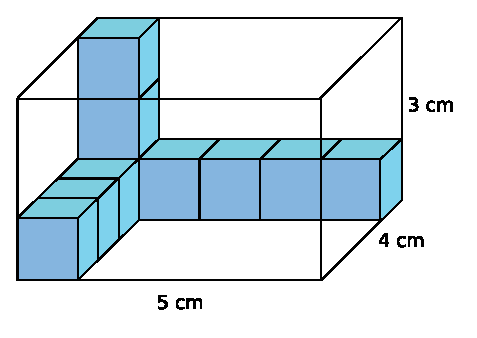
\includegraphics[width=7cm]{boite_remplir} \end{center}
\begin{enumerate}
 \item Combien de cubes faut‑il pour remplir le fond de la boîte ?
 \item En comptant les cubes déjà dans la boîte, combien de couches faut‑il pour remplir toute la boîte ?
 \item En comptant les cubes déjà dans la boîte, combien de cubes faut‑il au total pour remplir toute la boîte ?
 \item Déduis‑en le volume de cette boîte.
 \end{enumerate}
\end{partie}

\begin{partie}
Reprends les questions précédentes avec une boîte de dimensions 9 cm, 10 cm, 12 cm.
\end{partie}

\begin{partie}
Quelles dimensions doit‑on connaître pour calculer le volume d'un parallélépipède rectangle ? Déduis‑en une formule permettant de le calculer.
\end{partie}

\end{activite}

%%%%%%%%%%%%%%%%%%%%%%%%%%%%%%%%%%%%%%%%%%%%%%%%%%%%%%%%%%%%%%%%%%%%%%%%%%

\begin{activite}[Conversions]

\begin{partie}
Un parallélépipède rectangle a pour dimensions 4 cm, 6 cm et 8 cm.
\begin{enumerate}
 \item Quel est son volume en cm\up{3} ?
 \item Combien faut-il de cubes de 1 mm d'arête pour le remplir ?
 \item Quel est son volume en mm\up{3} ?
 \item Quelle opération doit-on effectuer pour passer du volume d'un solide en cm\up{3} à son volume en mm\up{3} ?
 \end{enumerate}
\end{partie}

\vspace{2em}

\begin{minipage}[c]{0.8\linewidth}
\begin{partie}[Une petite expérience]
\begin{enumerate}
 \item Trouve un récipient de forme parallélépipédique. Mesure ses dimensions et calcule son volume en dm\up{3}.
 \item Quelle est la \textbf{capacité} de ce récipient en litres ? (Si elle n'est pas indiquée sur le récipient, tu pourras le remplir d'eau puis mesurer sa capacité à l'aide d'une éprouvette graduée.)
 \item Déduis-en alors la correspondance entre un volume en dm\up{3} et une capacité en litres.
 \end{enumerate}
\end{partie}
 \end{minipage} \hfill%
\begin{minipage}[c]{0.16\linewidth}
 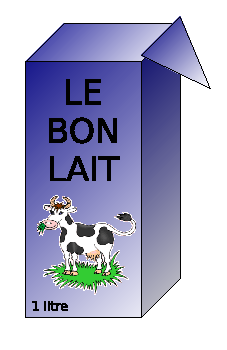
\includegraphics[width=2.5cm]{bon_lait}
\end{minipage} \\

\end{activite}

%%%%%%%%%%%%%%%%%%%%%%%%%%%%%%%%%%%%%%%%%%%%%%%%%%%%%%%%%%%%%%%%%%%%%%%%%%
